\chapter{Resource Allocation on Grid Systems}
\addcontentsline{toc}{chapter}{\numberline { }Bibliography}
\addcontentsline{toc}{chapter}{\numberline { }Bibliography}
\label{CHAPTER:GRID}
\centerline{\rule{149mm}{.02in}}
\vspace{2cm}

%%%%%%%%%%%%%%%%%%%%%%%%%%%%%%%%%%%%%%%%%%%%%%%%%%%%%%%%%%%%%%%%%%%%%%%

\section{The Grid Concept}

Since the invention of the computer, there has always been a demand for more
computational performance and resources. Initially this was met by the
development of faster machines and more efficient software. The continued
demand for more performance led to the use of many faster machines in parallel, and now we
have massively parallel clusters of commodity hardware, with a recent move to
multiple processors on a single chip. And while the average desktop computer
today has sufficient performance to handle the demand of a typical user, there
are still many users that require more computational power. 

To meet these needs, organisations often build large high performance computing
(HPC) systems, which are capable of much higher computational performance.
However, the cost of these HPC resources is significant.  They are increasingly
in demand, but the hardware is expensive to buy, maintain and run.  Initial
hardware costs can be millions of pounds, and the recurring costs, such as
power, cooling, repairs, parts, and floor space can add up to a non-negligible
monthly sum. And the larger the resource, the more skilled staff are needed to
keep it running smoothing, adding significant salary costs.  This means that
only those with sufficient resources (large companies or institutions) can
feasibly make use of HPC resources.

These high costs lead to organisations looking to utilise their existing
infrastructure as much as possible. Many make use of the spare computation
available on idle resources, such as utilising staff desktops overnight. This
also has an administration overhead, but can be more cost-effective than a
purpose built HPC resource.

If computational resources were able to be utilised, and made available to
users as a utility service, the demand for performance could be better met.  On
one hand, it would lower the barrier of entry for everyone, allowing modestly
resourced organisations to access previously unavailable computing power. On
the other, it would allow multiple HPC resources to be used simultaneously,
which would allow for very large problems to be tackled, that otherwise would
be Computationally infeasible. It would also allow new kinds of services to be
built upon previously unavailable on-demand access to HPC resources.  

Also, it would help mitigate the costs of providing the resources, as they
could potentially gain a better return on their investment and increased
resource utilisation. Office machines could be made available overnight,
providing a large pool of cheap computational power.

This is the idea behind the grid, providing HPC resources as a utility for
many.  It has also been called Utility Computing by some, autonomous
computing by others, but they are largely synonymous.

The idea of a grid is a relatively recent concept, even in the fast moving
world of computer technology.  It draws its inspiration from previous 'grids'
that have developed, such as transport, telecommunication and power grids.
These 'grids' supply affordable, scalable and powerful resources to the whole
of modern day society. The resource `the grid' will supply is main computational
power, but also storage, network and specific application resources.

There will be other uses that are currently beyond our conception and vision.
Governments, corporations, academic institutions and organisations will all be
able to make productive use of grid technology.  These capabilities elevate the
grid to an important research area, and it has received much attention over the
last decade.



%%%%%%%%%%%%%%%%%%%%%%%%%%%%%%%%%%%%%%%%%%%%%%%%%%%%%%%%%%%%%%%%%%%%%%%


\section{History of Grid Research}
\label{SEC:GRID:HISTORY}

The term ``The Grid'' was made popular in 1998 with
\cite{grid-foster99-blueprint}, which defined a grid as ``a hardware and
software infrastructure that provides dependable, consistent, pervasive, and
inexpensive access to high-end computational capabilities''.  This book was
quickly followed by \cite{grid-foster01-anatomy} .  This work looked to
identify the grid concept and start to define it in more detail.

However, there had been much work prior to this by various groups working on
various utility computing projects, and then grid concept had emerged out of
all these projects.

\subsection{Early Work}

The earliest effort was Condor\cite{grid-basney99-condor} , based at the
University of Wisconsin.  It was designed to make use of idle workstations to
run independent jobs. If a workstation ceased to be idle, the job would be
'frozen' and migrated to another machine to continue.  It was the earliest
example of a fault-tolerant allocation algorithm (see
\ref{SEC:GRID:ALLOCATION}, and made use of the
ClassAd\cite{grid-raman98-classad} system for matching jobs to resources. It is
still under development, having being 'modernised' with current grid concepts
as Condor/G\cite{grid-frey01-condor-g}.

Legion\cite{grid-chapin99-legion} was started in 1993, and based on an Object
Oriented view of the system. It presented the grid as a giant virtual machine
to the user with which to execute jobs. Originally based at the University of
Virginia, it was commercialised via Avaki Corporation as a complete grid
infrastructure, and has had some success, recently being bought out by database
providers Sybase.

The Unicore\cite{grid-romberg99-unicore} project started in 1997 and was
developed to provide access to HPC resources all across Germany. Like Legion,
it is a complete grid implementation, implemented in JAVA, providing access
through a single gateway, hiding much of the complexity from the user. 

The leading grid implementation is the Globus\cite{grid-globus-www} project, a
collaboration of many organisations. It provides a toolkit to implement many of
the low-level grid services, such as security, but leaves a lot of room for
development of higher level services and applications. Originally released in
1998\cite{grid-foster98-globus}, the Globus Toolkit\cite{grid-foster06-toolkit}
is now at version 4 and counting, and has been adopted as the defacto standard
grid implementation.

The key innovations demonstrated by these applications are that of use of
multiple disparate HPC facilities, with different architectures and locations,
connected using current networking technologies, as well as the automatic
allocation of resources on these machines. These were the early attempts at
implementing grid systems.

\subsection{The Open Grid Forum}

The multiple grid-orientated projects around the world prompted the need for
standards and specifications for grid systems. The Global Grid Forum
(GGF)\cite{grid-ggf-www} formed in 1999 to be a focal point for the emerging
grid concepts and technologies, and a place for these different groups to work
together on defining and building grid systems. The project has since rebranded
itself as the Open Grid Forum (OGF).

One of the initial key proposals that came out of the OGF was the Open Grid
Services Architecture (OGSA)\cite{grid-foster05-ogsa}, and its underlying
infrastructure, the Open Grid Services Infrastructure
(OGSI)\cite{grid-tuecke05-ogsi}. This was an initial attempt to draw up an
overall pattern for grid development. However, it revealed that key
interoperability technologies were needed in order to implement grid systems.

In the web world the idea of Web Services (WS)\cite{grid-ws-www} was gaining
interest as an interoperability solution. Based on the
SOAP(\cite{grid-soap-www}) protocol, WS (in theory) allowed remote procedure
call between any systems supporting the WS standards.

The OGF decided to utilise the WS standards as the solution to their
interoperability challengers and in 2002 refactored the OGSA to use
WS\cite{grid-czajkowski04-refactor}, and released as the Web Service Resource
Framework (WSRF)\cite{grid-czajkowski04-wsrf}.  It defined the standard
services a grid would need to function, and the interfaces between them. 
Additionally, the basic WS standards alone were not enough to implement the level of
interaction needed for grid computing. Particularly the lack of
\textit{stateful} resource access was a critical limitation. The OGF continures
to work with in partnership with the W3C\cite{grid-w3c-www} to add stateful Web
Services which would allow Web Services to be a standard way to implement the
WSRF services need for a grid system. All of the major grid middleware
applications are working towards providing the services described by OGSA via
the WSRF standards.



%%%%%%%%%%%%%%%%%%%%%%%%%%%%%%%%%%%%%%%%%%%%%%%%%%%%%%%%%%%%%%%%%%%%%%%

\section{Grid Challenges}

The grid introduces a whole new level of diversity to the problem of HPC resource
allocation.  The level of heterogeneity in capacity, type, location, and ownership is
much greater than in previous systems.

In order for this to be used on a large scale, any grid system would have to
provide a service that was transparent, reliable, and affordable, like any
other utility.  A common analogy for the concept is the UK's National Power Grid. A
user does not care which power station their electricity comes from, or the
technology of the generator, or which overhead lines it travelled down, nor
that it needs to be transformed before being supplied to their house. They are
simply concerned that its there when they plug in and switch on.  The
generation and supply of the power is transparent to them. If they had to
select and negotiate all the above factors, or if the supply was erratic and
unreliable, or overly expensive, they may seek other sources of power.

An additional factor present in grid computing that our National Grid analogy
does not capture is that of security. As information is now the resource being
supplied, a grid system would need to ensure secure delivery and receipt of the
workload and its results, whatever they may be. Individuals, both users and
suppliers, would need to be authenticated and authorised, this in itself no easy
task.

The grid is effectively a new model of computing, and as such there are many
challenges to overcome, in both understanding and implementation.  Some of the
challenges include : 

\begin{itemize}

  \item{\emph{Applications}} : Currently applications are designed mainly
    around single systems.  Many of the design methodologies, tools and
    environments are based on sequential systems.  While there has been much
    work done on parallel software, it remains a specialist field.  If grid
    enabled applications are going to be developed, then parallel programming
    models, tools and environments are going to need greater development.

  \item{\emph{Systems}} : The level of distribution and communication on a grid
    would be much more than current architectures handle, and the routers and
    load balancing systems that control a grid will need to be able to handle
    this dramatically increased load.   Networking protocols and infrastructure
    will also need much development if they are to be able to deliver the
    transparent access required. QoS must be provided for a grid system to
    function.

  \item{\emph{Algorithms}} : Problem solving algorithms, that utilise the
    distributed nature of the grid to solve the problems, will need to be
    developed in order to make the most of the grid environment.

  \item{\emph{Resources}} : Given the multitude and variety of tasks that will
    be run on a grid system, resource handling is a key issue.  The sort of
    resource managment that will need to be done is different in scale to the
    low-level management technologies so far, and much work will need to be
    done in this area, particularly in large scale co-allocation and
    reservation.

  \item{\emph{Security}} : With the orders of magnitude increase in data
    transmission that a grid will bring, security is of even more importance
    than ever before, and is a significant challenge.  Given the diverse
    ownership of grid resources, this poses an even bigger problem.

  \item{\emph{End user systems}} : Both the hardware and software design and
    implementation of end user system will have to change in order to adapt
    them to be part of a grid.  Current designs are based on being a single
    entity, and much work needs to be done in grid enabling these systems.

\end{itemize}



%%%%%%%%%%%%%%%%%%%%%%%%%%%%%%%%%%%%%%%%%%%%%%%%%%%%%%%%%%%%%%%%%%%%%%%%%%%%%%

\section{Grid Applications}
\label{SEC:GRID:TYPES}
A grid is a meta-computer on which applications can be run.  It is the
applications that provide the useful information and services that are the
reason for the existence of the grid in the first place.

\subsection{Types of Application}

A brief synopsis of the various general types of applications that will be run
on a grid system, is given in \cite{grid-foster99-blueprint}.  It is summarised
and illustrated here.

\begin{itemize}

  \item{\emph{Distributed super-computing}} - also known as Grand Challenge
    applications, these solve very large or intensive problems that require
    either many processors (for speed) and/or vast amounts of memory (for large
    problem sizes). Many of the existing grid systems and their applications
    are based on solving these kinds of problems.

  \item{\emph{High throughput}} - utilising idle systems to increase the
    aggregate throughput of an existing application.  Examples include
    micro-processor chip verification at idle engineers workstations.  The
    Condor system\cite{grid-basney99-condor} utilised idle workstations to
    perform a variety of compute intensive tasks.

  \item{\emph{On demand}} - applications which dynamically allocate specific
    resources for a particular period upon request, for a specific purpose.
    Good examples are medical procedures that can utilise real-time image
    processing through on demand allocation of computational resources.

  \item{\emph{Data intensive}} - processing vast amounts of data and
    synthesising new information.  The processing of high energy physics
    experiment results requires terabytes of data to be processed in small time
    scales.

  \item{\emph{Collaborative}} - applications that allow collaborative working
    between multiple distributed parties.  This includes the virtual laboratory
    concept.

\end{itemize}

Some applications may be of more than one type, but these are the various
uses of grid systems that we can currently see.  Again, others may emerge as
the field matures.

\subsection{Types of Grid Systems}

The actual purpose and function of specific grid systems may vary widely
depending on their creators desires.  One grid may not function the same way or
for the same reason as another. Krauter \textit{et al}
\cite{grid-krauter02-taxonomy} classify potential grid systems into three main
categories, depending on function and purpose.

\begin{itemize}

  \item{\emph{Computational Grids}} - grid systems that have higher
    computational capacity for a single application than any component machine.
    This will replace the current stand alone super-computer idea, and allow
    extremely demanding applications to be run in practical time scales and
    with much larger problem sizes than previously possible.

  \item{\emph{Data Grid}} - an infrastructure for storing, analysing and
    synthesising new information from data repositories.  Similar in nature to
    a computational grid, but its focus is specifically on the storage and
    management of huge amounts data.

  \item{\emph{Service Grid}} - these are grid systems that provide computing
    services that are not available from a single machine.  It provides an `on
    demand' service to the user, such as interactive multimedia and
    collaborative conferencing.

\end{itemize}

All three categories of grid system will use the same underlying network and
computing technologies, but the way in which resources are managed and
allocated will be very different, and the intended usage and user groups are
also diverse.  For example, it can be expected at the current time that the
main users of computational grids will be the academic community and a small
section of industry.  The cost effective availability of these super computing
resources may however induce more interest and use from the industrial sector.
It is unlikely that any consumer will use its facilities directly. A service
grid, however, does have potential for large scale use in the consumer market,
especially the multimedia possibilities. It may be that other types of grid
system emerge in the years ahead - it is still a new and largely undeveloped
area.

Another distinction in grid types is less technical and more social in origin.
The grid concept has largely been developed in academia, which is an open and
public environment. The typical applications for HPC in academia are open and
freely available anyway, so data security in not a big concern. In industry,
however, this is often not the case. Companies can have large amounts of
proprietary data that they wish to keep private, and as they would not own the
resource that would execute their application, would not be able to guarantee
their data's integrity. Any disgruntled local system administrator could
potentially spy on the applications execution. This leads to the possibility
of ``open grid'', which are the normal kind, and ``closed grids'', which are
hired wholesale (or in isolated sections) from a trusted provider.

%\subsection{Typical Use Cases}

%globus paper

%classes of application (e.g. parameter sweep)



%%%%%%%%%%%%%%%%%%%%%%%%%%%%%%%%%%%%%%%%%%%%%%%%%%%%%%%%%%%%%%%%%%%%%%%%%%%%%%


\section{Architecture}

The architecture of a grid is decomposed into distinct layers, similar to the
current networking protocols on which they are based.  Figure
\ref{FIG:GRID:ARCH} is taken from \cite{grid-foster01-anatomy} and describes a
high level view of the current grid architecture.

\vspace{1cm}
\begin{figure}[h] 
  \centering
  \fbox{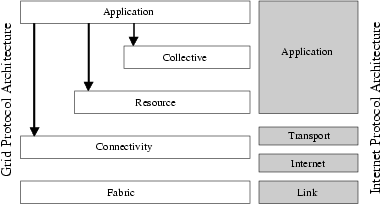
\includegraphics[width=14cm]{grid/grid-arch.png}}
  \caption{Grid architecture protocols with corresponding internet protocols
           (from Foster \textit{et al} \cite{grid-foster01-anatomy})} 
  \label{FIG:GRID:ARCH}
\end{figure}

We examine each of these layers in turn, starting from the bottom up. This grid
'layer' model bears much similarity to the original OSI reference
model\cite{grid-osi-www} for the internet.

\subsection{Grid Fabric Layer}

The elements at this layer comprise of the actual resources of the grid system,
as well as the low-level interface to the resources themselves.  Given their
heterogeneous nature and differing administration policies, this is not a
simple task.

The available resources can be broken down into three main types of resource.

\subsubsection{Computational Resources}

These are the actual computers that do the work. In
\cite{grid-foster99-blueprint} four basic system types are suggested.

\begin{itemize}

  \item{\emph{End user systems}} :  These are what is commonly meant by the
    word 'computer'.  They represent the smallest grid 'unit'.  They also
    include storage systems and sensors.  They are tightly designed in function
    as a single entity with hardware and software designed to work together in
    a homogeneous environment.

  \item{\emph{Clusters}} : A cluster is a network of systems that is
    specifically designed to be used as a single high powered computational
    resource.  Like an end user system, clusters are most often highly homogeneous
    and have a single controlling entity through which resource requests are
    made.  They have arisen as a more affordable, scalable and possibly more
    powerful alternative to traditional integrated supercomputers.

  \item{\emph{Intranets}} : These are large local networks belonging to a single
    organisation.  They are generally heterogeneous in nature, with a large
    variety of resources available.  Different parts of the system may be under
    different administration and there is less global knowledge about the
    system than in either a cluster or end user system.

  \item{\emph{Internets}} : These are large networks spanning multiple
    organisations.  These are even more heterogeneous in nature than intranets,
    and have even less global knowledge available.  They often are much more
    geographically distributed also, increasing latency and other communication
    issues.

\end{itemize}

These are the systems that a grid will be constructed from.  Whether dedicated
to grid usage or used when idle, these systems will actually do the computation
that the grid offers.

\subsubsection{Storage Resources}

These consist of dedicated storage machines optimised for fast efficient
storage. They can also include dedicated databases for querying or updating,
holding pre-processed data for use by many applications.

Given the vast quantities of data that a super-computing application can
produce (in the order of GB/s), the capability to store and later retrieve and
process this data is very important.


\subsubsection{Network Resources}

These resources are not the actual transmission and network devices, but rather the
facilities they provide, i.e. connection and bandwidth.  Achieving Quality of
Service (QoS) is very important for grid systems as they rely heavily on fast
communication.  It will be necessary for a grid system to be able to reserve
and allocate network resources such as bandwidth on a whole variety of
different network structures and capacities.



\subsection{Grid Connectivity Layer}

This layer is responsible for all aspects of actual connection between grid
components.  As well as the actual data and message transmission, it is
responsible for the authentication of user and request, i.e. that they are
allowed to use a particular resource.  It is also responsible for security of
transmission and the integration with diverse security policies and procedures
on different resources.  It must also track usage and keep account of
resources used for each application, for determining costs incurred. The
development of this layer is very much linked with the development of Internet
technologies such as IPv6 and other QoS mechanisms.


\subsection{Grid Resource Layer}

This layer controls the reservation and allocation of a single resource, as
well as taking responsibility for the execution of jobs on that resource.  It
is unconcerned with anything other than the resource management, and is unaware
of the global state of the grid.  It provides information on the state, load,
usage and free capacity of its own resources.  It also allows direct management
of applications executing on its resources, such as process creation,
monitoring and reporting.


\subsection{Grid Collective Layer}

This is the layer that pulls all the resources together coherently.  It allows
access to and maintenance of a grid wide information service that can provide
the state of any resource on the grid.  This allows it to co-reserve and
co-allocate resources across the whole grid.  It is concerned with the
concurrent management of all the resources available to the grid

\subsection{Grid Application Layer}

This is similar to the internet application layer at the highest level.  These
are the applications written by users to run on grid systems.  They use the
other grid layer protocols to acquire and use the resources they need.  An
`application' may actually be a grid `portal' or entrance for another specific
type of application.


The area this study concerns is the Collective layer. This is where the
details of the resource allocation are worked out, and we look at the aspect in
more detail. 




%%%%%%%%%%%%%%%%%%%%%%%%%%%%%%%%%%%%%%%%%%%%%%%%%%%%%%%%%%%%%%%%%%%%%%%%%%%%%%


\section{Resource Discovery and Allocation}
\label{SEC:GRID:ALLOCATION}

The focus of this thesis is on a novel mechanism for resource allocation, and it
is to this area of grid research that we will look at in detail.

HPC is not new, and many successful systems and technologies have been
developed to manage the usage of the resources. Typically, a HPC resource is a
single multi-processor parallel machine, or a cluster of many smaller machines.
They are usually owned by a single organisation, although there may be many
different groups of users within the larger body, and are usually based at a
single location, rather than spread between several sites. 

Grid scheduling has seen much development recently, for an in depth review see
\cite{grid-nabrzyski04-review}.  In current grid implementations, resource allocation is broken
down into two main steps, resource discovery, and resource selection or
allocation. Resource discovery is the process of knowing what resources are
available for use, as well as their current load and state, whereas resource
allocation in this sense mean the actual determination of which resource to
execute an application on.

\subsection{Resource Discovery}

The dominant resource discovery provider is the Globus Toolkit's Meta-Directory
Service (MDS) \cite{grid-czajkowski01-mds2} which has been developed since the
projects inception, and has undergone several major revisions as the OGF
specifications have developed. It supplies a grid directory service and a
protocol for querying the service for information about a resource or set of
resources, in order to aid a user or application to select suitable resources
to use. The directory maintains itself by both allowing registered resources to
push information to the service and regularly pulling this information from the
resources. Entries in a directory have a limited lifespan and must be renewed
periodically or be removed from the directory. The design facilitates multiple
directory servers that aggregate resource information, as a resource could be
registered on multiple independent directories. This is aimed at increasing
scalability and robustness, which has been a limitation and subject of
investigation\cite{grid-iamnitchi01-agent}.

There is an inherent trade-off between the accuracy of information in a
directory about a resource's state, and the number of resources registered. The
more frequent the updating of state to the directories, the more accurate the
grid information will be, but the greater the demand on the directory services.
In a typical MDS deployment, of a few hundred resources, a directory's
information is out of date by about 5 minutes. This is suited to grid
environments where the demand is relatively stable and jobs are long running.

MDS provides the infrastructure on which grid meta schedulers could allocate
grid resources, but does not implement any such algorithms itself. Often its
left for specific applications or users to make final decisions. It is not a
complete allocation mechanism, but provides and important service upon which to
build such a mechanism.

\subsection{Resource Selection/Allocation}

Typical grid level allocation and scheduling query a directory service and
perform some kind of algorithm on the query results to select the resource to
be used.

Many schedulers are design to schedule jobs on local resources under a single
domain. Condor-G\cite{grid-frey01-condor-g} is a dynamic on-demand scheduler
for dedicated and idle resources. Sun's GridEngine\cite{grid-bulhoes04-sge}
uses a sophisticated priority queuing system and supports advance reservations.
The Portable Batch System (PBS) \cite{grid-henderson95-pbs} is one of the
oldest schedulers around, but has been adapted to suit more modern
environments. The most common commercial system is the Load Sharing Facilitator
(LSF)\cite{grid-lsf-www}, which is widely deployed. These system are often used
to aggregate a group of heterogeneous resource to present a single resource
interface to a larger grid system.

The EZ-Grid project\cite{grid-chapman01-ezgrid} and the Grid Resource
Broker\cite{grid-aloisio02-grb} gather grid information and help users make
allocation decisions, but do not actually schedule anything automatically.

There are actually very few functional grid-level schedulers. AppLeS
(Application-Level Scheduling) \cite{grid-berman03-apples} can schedule jobs
in highly heterogeneous and dynamic environment. The Maui scheduler
\cite{grid-maui-www} has good provision for advance reservation and QoS. The
Gridway project \cite{grid-gridway-www} provides a full scheduling system, with
fault tolerance and job migration. It uses the Globus toolkit and focus on
interoperability between different local schedulers.

Of particular relevance to this study is the
Nimrod/G\cite{grid-buyya00-nimrod-g} project, which is based on an economic
paradigm. It is specifically designed for easily parallelisable parameter sweep
applications, and is built upon the Globus Toolkit. It allows users to
negotiate prices and completion deadlines, including advance reservations.  See
section \ref{SEC:ECON:GRIDECON} for a more detailed discussion.


\subsection{Limitations of Centralised Approaches}

The current approaches have been developed out of the traditional HPC field,
and have facilitated initial grid implementations. They are all centralised in
nature, as this is the most straight forward implementation.  However, they
face some serious challenges as the size and use of grid systems continue to
increase.

\begin{itemize}

  \item Scalablity. The chief challenge in building grid systems is size. Once
    a grid consists of more than a few hundred machines, current grid systems
    struggle to cope. If the full potential of grid systems is to be acheived,
    breakthroughs in improving scalability are essential.

  \item Dynamism. Different grid usage demand levels mean different policies
    and usage patterns. Current grid systems are not designed to adapt to high
    degrees of change in demand (and conversely, supply). If resource state is
    changing more rapidly than a centralised directory can keep up with, the
    accuracy of information is decreased, leading to incorrect allocation
    decisions being made. This can lead to decreased performance of both the
    allocation system and the grid resources themselves, as more work is needed
    to successfully allocate jobs, and more load on the allocation system,
    which can spiral downhill.

  \item Single Point of Failure. Whilst this has been addressed to some degree
    by systems such as MDS, any centralised system, even if aggregated, is
    vulnerable if the central mechanism fails in some way. If it fails
    completely, the system may be totally unusable. If it's performance starts
    to degrade, the whole system's performance suffers.

\end{itemize}

Whilst there is much investment and knowledge in such centralised systems, and
much work still to be done based on that paradigm, there are inherent
limitations. Therefore it is important to explore decentralised approaches as
potential solutions to this problem, as the limitations of centralised systems
are the strengths of decentralised systems. And it is specifically these
limitations which grid computing it trying to overcome. 



\section{Summary}

The grid has definitely been conceived and born.  How far along it is in its
development is not clear, although its is still in its infancy.  Much work has
been done on existing technologies and their application to the grid.  Work has
also been done in identifying the issues involved with enabling a grid scale
computing system.  Resource co-allocation is a key issue in this work, and is a
relatively little developed field.

As well as investigation into grid management technologies, research into the
underlying technologies must also continue.  If the grid concept, as envisioned
and stated by it proponents, is to become reality, large advances in the fields
of networking transmission speeds, network management, parallel software
development and parallel hardware are necessary.

However, the potential is clear. In the short time the grid has been conceived,
interest has grown considerably.  This is due to what the grid could provide
for scientists of many disciplines, and maybe eventually to mainstream
consumers. Like the National Grid before it, it could dramatically impact the
quality of life for many people life.
